%---------------------------------------------------------------------------%
\lecture{Research Presentation}{lec_present_application}
%---------------------------------------------------------------------------%
\section{Data Application}%
%---------------------------------------------------------------------------%
\begin{frame}[fragile]
    \frametitle{Prostate Cancer Data Set}
    \begin{itemize}
        \item What is the relationship between log prostate specific antigen (lpsa) levels, which is elevated in men with prostate cancer, and other clinical measures $(p=8)$
        \item $n=97$
        \item For comparability we use the same train-test split as \cite{zou2005regularization}
        \item High correlation between
            \begin{itemize}
            \item lcp \textit{(log of capsular penetration)} and lcavol \textit{(log cancer volume)}
            \item svi \textit{(seminal vesicle invasion)} and lcp
            \item pgg45 \textit{(percent of Gleason score 4 or 5)} and gleason \textit{(Gleason score)}
            \item pgg45 and lcp
            \end{itemize}
    \end{itemize}
\end{frame}
%---------------------------------------------------------------------------%
\begin{frame}
\frametitle{Correlation Matrix}
    \begin{figure}
    %\column{.5\textwidth}
        \centering
        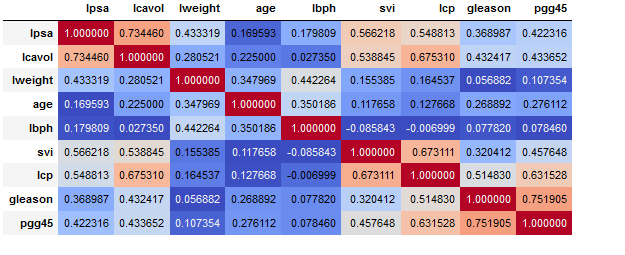
\includegraphics[width=11cm,height=5.5cm, left]{Img/corr_table.png}
    \end{figure}
\end{frame}
%---------------------------------------------------------------------------%
\begin{frame}
%\begin{columns}[t]
%\column{.5\textwidth}
\centering
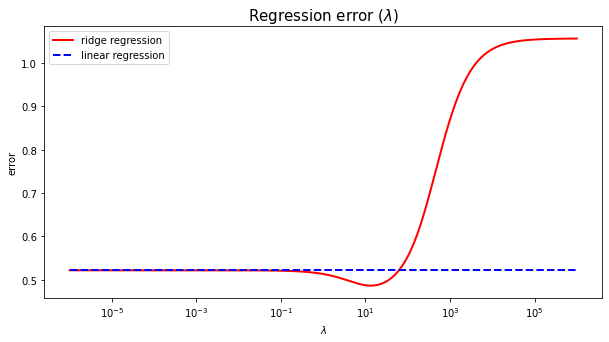
\includegraphics[width=7cm,height=4cm, left]{Img/data_ridge_vs_lambda.png}
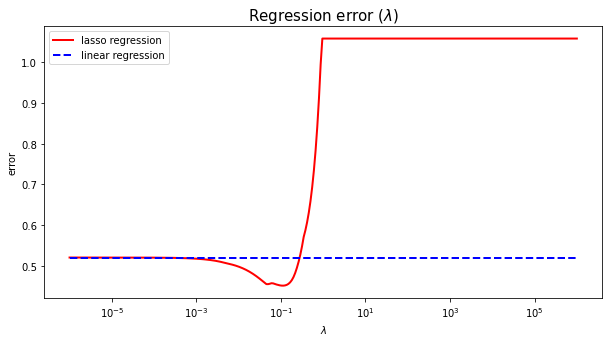
\includegraphics[width=7cm,height=4cm, right]{Img/data_lasso_vs_lambda.png}\\
%\column{1.0\textwidth}
\centering
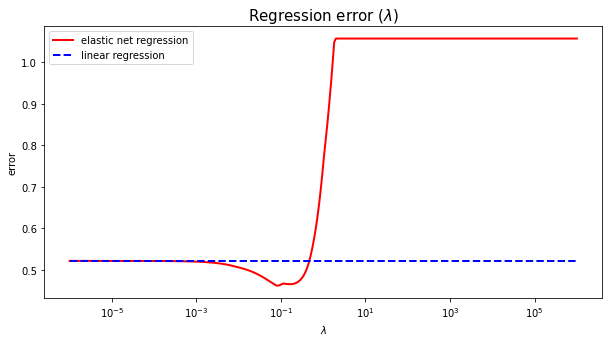
\includegraphics[width=7cm,height=4cm, center]{Img/data_elnet_vs_lambda.png}\\
%\end{columns}
\end{frame}


%---------------------------------------------------------------------------%
\begin{frame}
%\begin{columns}[t]
%\column{.5\textwidth}
\centering
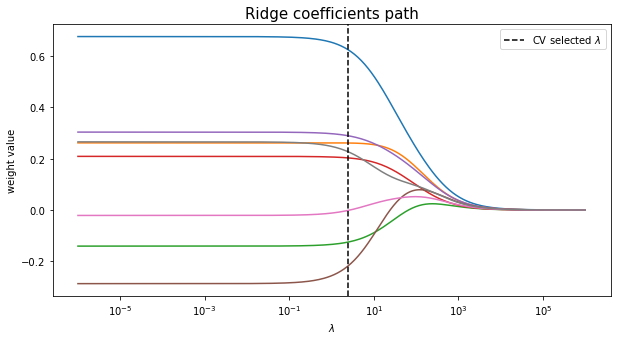
\includegraphics[width=7cm,height=4cm, left]{Img/data_ridge_coef_path.png}
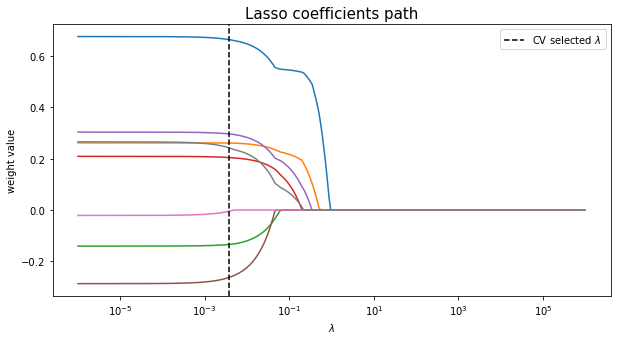
\includegraphics[width=7cm,height=4cm, right]{Img/data_lasso_coef_path.png}\\
%\column{1.0\textwidth}
\centering
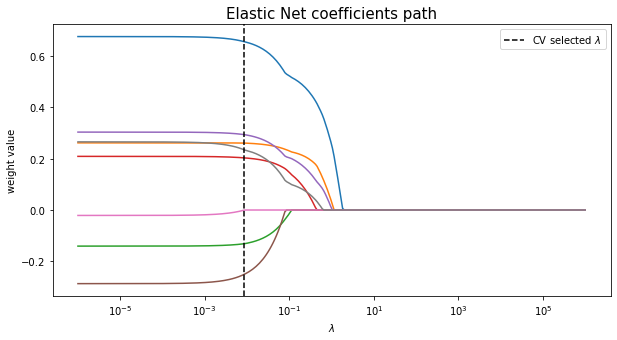
\includegraphics[width=7cm,height=4cm, center]{Img/data_elnet_coef_path.png}\\
%\end{columns}
\end{frame}

%---------------------------------------------------------------------------%
\begin{frame}
\frametitle{Model Selection}
\begin{center}
\small
\begin{tabular}{||c c c c||} 
 \hline
 Model & Test MSE (with 10-fold CV) & Test MSE (AIC) & Variable Selection\\ [0.5ex] 
 \hline\hline
 Linear & 0.5213 & - & All\\ 
 \hline
 Ridge & 0.5043 & - & All\\
 \hline
 Lasso & 0.5112 & - & All\\
 \hline
 Elastic Net (Naive) & 0.5043 & - & All\\
 \hline
 LARS & 0.5084 & 0.5033 & lcavol, lweight, lbph, \\ & & & svi, pgg45\\
 \hline
\end{tabular}
\end{center}\\

\begin{block}{Takeaway}
\begin{itemize}
\item Naive elastic net performs as well as ridge, also reported by \cite{zou2005regularization}
\item Lasso performs best if LARS algorithm is implemented and AIC is used for tuning $\lambda$. It performs variable selection as in \cite{zou2005regularization}.
\end{itemize}
\end{block}

\end{frame}